\section{Previous Work}
\label{sec:previous_work}

As mentioned before, the goal of this project, besides to gather new knowledge
about the conjunction of \ac{HPC} and \ac{CC} is to extend the result of a previous project
by enabling it to become an Interactive Supercomputing Environment.

But as we will be take this previous system as a basis for our prototyping,
we will need to understand the design and architecture of the existing system,
and then decide which parts will be extended, which will be replaced, which will be removed
and which will be kept as they are.

The goal of the previous project was also a converged \ac{HPC} system based on the \textit{Arkouda} library,
but instead of focusing on an interactive environment,
it is based around a \gls{GitOps} workflow, where instead of the user interacting with the system directly,
the user submits code to a central version-control-system,
from where it gets cloned and packaged into container automatically.
If certain predefined conditions are met the workflow-system will then start
the container on the cluster and execute the code.

\pagebreak

\section{Existing Infrastructure}
\label{sec:existing_infrastructure}

\begin{figure}[!ht]
    \vspace{0.8cm}
    \centering
    \scalebox{0.35}{
        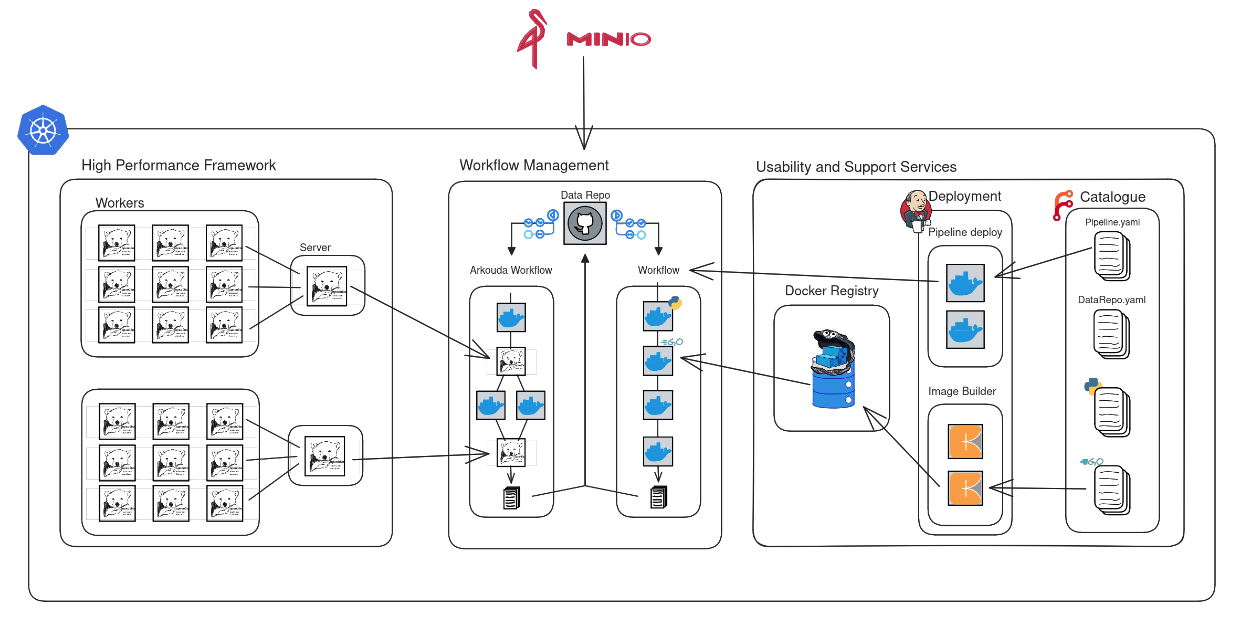
\includegraphics{./graphics/Pachykouda - High level architecture.png}
    }
    \caption{High level architecture of Pachykouda\protect\footnotemark}
    \label{fig:pachykouda_architecture}
\end{figure}
\footnotetext{Taken from \cite{eckerthDevelopmentDemonstrationProofofconcept2023}}

In the figure \ref{fig:pachykouda_architecture} we can see the high level architecture of the existing system,
it is split up in three relevant sections:

\begin{itemize}
    \item \textbf{Usability and Support Services:}  On the most tightern side we have the supporting infrastructure which also runs on the Kubernetes cluster,
          this includes the versioning system (Forgejo), the agent which builds the containers and workflows (Jenkins)
          and the storage for the containers images (Registry V2).
    \item \textbf{Workflow Management:} In the middle we have the workflow system(Pachyderm), which is responsible for the orchestration of the workflow,
          it starts the containers, manages their input and output and ensures the versioning of the results.
    \item \textbf{High Performance Framework:} On the left we have the Arkouda workers and the Arkouda server, which are the actual \ac{HPC} part of the prototype.
\end{itemize}

Beneath the service layer we have the Kubernetes cluster, which is responsible for the orchestration of the containers and managing the resources,
for both the computation as well as the all the other services, the only exception being the storage of the datasets versioned by
workflow system, which stores them in an external storage system, running on the a node of the same cluster, but not managed by Kubernetes.

On a hardware level we have a cluster of 20 nodes, connected by a 10Gbit/s network, in a star topology with a central switch.
Each node has a \textit{Intel Xeon E5-2680 v3 (48) @ 3.300GHz} and 270GB of RAM according to the information given in
the system stats. Also five of the nodes actually have an Infiniband capable network card, which could be used to test
the functionality of \ac{RDMA} capabilities of the Arkouda library, or jobs only requiring few cores but a lot of bandwidth.
On the Network abstraction layer the cluster is using the \textit{Flannel} network overlay, which provides a simple
layer 3 network between the nodes\footcite{flannelFlannelioFlannel2024}.


\section{Implication for the Prototype}
\label{sec:implications_for_prototype}
In the section \nameref{suggested_architecture} we created a suggestion for an architecture based on
our deductive reasoning we have done during the deductive analysis, as we now have discussed the environment
and existing infrastructure, we can now assess how our theoretical architecture can fit in a real world scenario.

The largest section of the previous system is the workflow management and its supporting infrastructure,
while this is also able to access the compute resources provided by the \ac{HPC} part of the system,
from a structural standpoint it will not impair the function of the system we are planning to building.
And the already running container \gls{registry} will also be useful for our prototype, as we will be able to use it to store the images of the containers we will be using.
Instead it demonstrates the high flexibility of kubernetes, being able to run many different services on the same cluster.


The \ac{HPC} part of the system we will be using as a basis for our prototype.
It is already able to run the Arkouda library, even though it is as of right now only accessible  through the workflow system.
while there is potential for optimization and improvement, it will provide a solid foundation for our work.

On the other hand, the cluster is mostly connected through a non \ac{RDMA} capable network,
which will limit the performance of the Arkouda library as discussed before.
While we do have two nodes with Infiniband network cards, we will only be able to use them for testing purposes,
but not in a full scale production like environment.
While there is little we can do about the available hardware,
Another consideration is the \ac{CNI} currently in use on the cluster,
as we might want to use a multi network setup, in oder to provide a separate network for the \ac{RDMA} capable nodes,
we would need to install \textit{Multus} or a similar \ac{CNI} on the cluster, which we then combine
with and \ac{RDMA} capable \ac{CNI} like \textit{OVN4NFV} or \textit{SR-IOV}.

While not a total necessity, it might be beneficial to have a container runtime available,
which is closer aligned with the \ac{HPC} part of the system, such as \textit{Singularity},
as it brings additional features such as native \ac{GPU} support and \ac{MPI} support, which might be useful for the prototype.

\pagebreak